
\documentclass[12pt]{article}

\usepackage{sbc-template}

\usepackage{setspace}
\usepackage{graphicx}


\usepackage{amsmath,amsfonts,amsthm,amssymb}         % fontes matemáticas, teoremas e etc.
\usepackage{latexsym}                                % mais símbolos matemáticos
\usepackage{cancel}
%\usepackage[portugues,algoruled,lined]{algorithm2e}  % excelente ambiente p/ escrever algoritmos
\usepackage{tabularx}                                % tabelas com diversas formas
\usepackage{multicol}                                % tabelas com multiplas colunas
\usepackage{multirow}                                % tabelas com multiplas linhas
\usepackage{booktabs}                                % tabelas profissionais
\usepackage{longtable}                               % tabelas longas
\usepackage{dcolumn}                                 % tipos especiais de colunas
\usepackage{lscape}                                  % página no formato paisagem
\usepackage{graphicx}                                % diversas configurações de imagens
\usepackage[normalem]{ulem}
\usepackage{fancyhdr}

\usepackage{geometry}
\usepackage{chngpage}


\usepackage[brazil]{babel}   
\usepackage[utf8]{inputenc}

     
\sloppy

\title{Modelagem TCP}

\author{Alisson Barbosa, Anderson, Inácio Alves, Luis Ribeiro,\\
 Sérgio Correia, Sérgio Vieira, Vinícius Romão.}


\address{Mestrado Acadêmico em Ciência da Computação (MACC)\\
  Universidade Estadual do Ceará (UECE).
%  \email{\{alisson, sergio, sergiosvieira, vinicius.romao\}@larces.uece.br, 
%  anderson@ifce.edu.br, \{inacioc.alves, luisribeirolima, vilsonfn\}@gmail.com}
}

\begin{document} 

\maketitle

     
\begin{resumo} 
  Este trabalho apresenta de forma detalhada as modelagens matemáticas do protocolo
  TCP encontradas nas seções 5.3.1 e 5.3.2 do Livro ``High Performance TCP/IP Networking''\cite{hassan2004high}
  e publicadas em \cite{Mathis_97} e \cite{padhye1998modeling}.
\end{resumo}


\section{Modelo Periódico}
%Importando descricao da secao 1
%Este arquivo deve ser alterado pelos integrantes da respectiva equipe com o conteudo indicado abaixo.
%Equipe: Sergio Luis, Inácio

%Livro: Seção 5.3.1, p.129

%Inserir no arquivo \textbf{modelo\_periodico.tex} a descrição do modelo TCP
%periódico.
Este é o modelo mais simples para o TCP, que considera o padrão periódico na
dinâmica da janela de congestionamento e a perda de pacotes. Não é levada em
conta nenhuma versão específica do TCP, mas apenas a dinâmica comum a todas
estas versões, ou seja, a maneira como a janela decresce multiplicativamente a
cada perda periódica de pacote. Como estamos considerando o estado estacionário
(\textit{steady-state}), um tamanho de janela máximo $W$ é sempre atingido no
momento em que um pacote é perdido, e isso resulta na redução da janela pela
metade, ou seja, $\frac{W}{2}$. Além disso, a operação do sistema no estado
estacionário implica que as perdas de pacotes ocorrem com probabilidade
constante $p$, tal que, em média, $\frac{1}{p}$ pacotes são transmitidos na rede
entre cada perda de pacote. Lembrando que na perda de pacote, a janela é
reduzida. Também é importante lembrar que, como estamos considerando o estado
estacionário, significa que atingimos um padrão regular, que persiste por todo o
tempo, ou seja, não é levado em consideração a partida lenta
(\textit{slow-start}), por exemplo, mas apenas o estado final, estável, com o
tamanho máximo da janela já atingido.

Se plotarmos a variação da janela em função do tempo, no estado
estacionário, observaremos a forma ``dente de serra'' do TCP. Apesar do modelo
periódico ser menos realista, ele permite que derivemos uma propriedade
fundamental com relação ao desemprenho do TCP, que é conhecida como a
\textit{lei da raiz quadrada inversa de p}.

Devido à forma periódica da dinâmica da janela no estado estacionário, o
desempenho do TCP nestas condições pode ser derivado determinando o número de
pacotes transmitidos em um perído, e o comprimento do período. Como temos uma
probabilidade constante ($p$) para a perda de pacotes, o número de pacotes é
dado por $\frac{1}{p}$, como dito anteriormente, porque nós temos que transmitir
esta quantidade de pacotes antes que um pacotes seja perdido. Uma maneira
alternativa de se encontrar o número total de pacotes transmitidos em um período
é encontrar a área sob o rastro do tamanho da janela, o que é bem simples,
devido à forma trapezoidal do período:

\begin{equation}
Numero\ de\ pacotes = \frac{1}{2}\frac{T}{RTT}\left(\frac{W}{2} + W\right)
\end{equation}

Onde $T$ é o período entre as perdas detectadas. O tempo deve ser escalado pelo
$RTT$ (\textit{round-trip time}), já que a fonte TCP não envia pacotes
continuamente, e o tempo deve avançar pelo período de um RTT antes que um
conjunto totalmente novo de pacotes, contido pelo tamanho da janela, contribua
com o número total de pacotes transmitido. Como sabemos que o TCP aumenta sua
janela na taxa de um pacote por RTT durante sua fase de crescimento linear, o
tempo que leva para aumentar a janela de $\frac{W}{2}$ para $W$ é $T =
RTT \cdot \frac{W}{2}$. Logo, igualando o número total de pacotes transmitidos
durante esse período, temos:
\begin{align}
\frac{W}{4} \cdot \left(\frac{W}{2} + W\right) &= \frac{1}{p}\nonumber\\
\Rightarrow W &= \sqrt{\frac{8}{3p}}
\end{align}

Nós podemos agora achar a taxa média de envio $\bar{X}(p)$ da fonte TCP, que é o
número de pacotes transmitidos a cada período:
\begin{align}
\bar{X}(p) &= \frac{\frac{1}{p}}{RTT \cdot \frac{W}{2}}\nonumber\\
			&= \frac{1}{RTT} \sqrt{\frac{3}{2p}}
\end{align}

Este resultado é conhecido como a \textit{lei da raiz quadrada inversa de p}, e,
em particular, mostra que a taxa de transmissão de uma fonte TCP é inversamente
relacionada ao RTT e a raiz quadrada da probabilidade média de perda de um
pacote.



\section{Modelo de Perda de Pacote Detalhado}
O desempenho de uma conexão TCP está sujeito a fatores como perdas de pacotes indicadas por 
ACKs duplicados ou \textit{timeouts} e limitação do tamanho da janela de transmissão pelo 
destinatário. O objetivo desta seção é apresentar um modelo que leva em consideração todos 
estes fatores, sendo mais abrangente que o modelo da seção anterior que não considera os dois
últimos itens citados.

A primeira subseção apresenta o modelo considerando apenas a perda de pacotes devido ao 
triplo ACK duplicado. A segunda subseção acrescenta ao modelo a perda de pacotes devido à
ocorrência de \textit{timeout}. A terceria subseção considera os efeitos da limitação do 
tamanho da janela pelo destinatário.
%Importando subsecoes da secao 2
%Equipe: Vinicius, Luis Ribeiro
%Livro: Seção 5.3.2, p.131

\subsection{ACKs Duplicados}
A modelagem do protocolo TCP é feita sobre o algoritmo de controle congestionamento TCP Reno.
Neste algoritmo, após o \textit{Slow Start}, o tamanho da janela de congestionamento ($W$) é 
incrementado em $1/W$ a cada \textit{ACK} recebido e decrementado a cada indicação de perda 
de pacote percebida. O valor da redução no tamanho da janela varia de acordo com o tipo de indicação de
perda de pacote: triplo \textit{ACK} duplicado ou \textit{timeout}. No primeiro caso o tamanho
da janela é dividido pela metade do seu valor corrente, no segundo a janela é reduzida a um 
pacote. Nesta seção consideraremos que perdas de pacotes são indicadas apenas por triplos 
\textit{ACK's} duplicados (TD).

O comportamento do protocolo TCP é modelado em termos de rodadas (\textit{rounds}). Uma rodada
se inicia com a transmissão de $W$ pacotes de uma janela. Uma vez que todos os pacotes tenham sido 
transmitidos, o remetente passa a aguardar a recepção de \textit{ACK's}. O recebimento do primeiro 
\textit{ACK} marca o fim da rodada atual e início da próxima. Note que a cada rodada o tamanho da 
janela é incrementado em um pacote.

A figura \ref{fig:tdp_macro} apresenta o comportamento de uma conexão TCP, descrito acima, em mais detalhes. 
Defini-se período TD (TDP) como o intervalo entre duas indicações de perda de pacote por triplo \textit{ACK} 
duplicado (TD). Durante este intervalo, o tamanho da janela é incrementado de uma unidade a cada rodada. 
No fim de cada TDP$_{i}$ o tamanho da janela é dividido ao meio.

\begin{figure}[ht]
  \centering
  \includegraphics[scale=0.8]{./figs/tdp_macro.pdf}
  \caption{Evolução do tamanho da janela quando perdas de pacotes são TDs.}
  \label{fig:tdp_macro}
\end{figure}



%Este arquivo deve ser alterado pelos integrantes da respectiva equipe com o conteudo indicado abaixo.
\subsection{Timeouts}

Ainda não incluimos os efeitos dos timeouts na modelagem do TCP. Mas, esses efeitos têm que ser levados em conta, visto que ocorrem frequentemente. Muitas implementações de TCP dividem o tamanho da janela após receberem três ACKs duplicados. Entretanto, se um transmissor não recebe qualquer ACK duplicado, ou recebe menos do que três, um pacote é tido como perdido somente através do estouro do temporizador de retransmissão, o timeout. Quando ocorre um timeout, o tamanho da janela é reduzido para um e o limite da fase de partida lenta é mudado para a metade do tamanho da janela antes de a perda ter acontecido. O pacote perdido é retransmitido e o temporizador é mudado para o dobro do período de timeout anterior. Como ocorrem atrasos significativos na espera do timeout, a taxa de envio do TCP é significativamente reduzida. \cite{hassan2004high} e \cite{padhye1998modeling} adaptaram o modelo detalhado de perdas de pacotes para demonstrar essa consequência.

\begin{figure}
\begin{center}
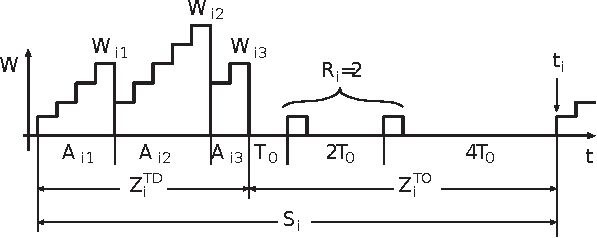
\includegraphics[scale=0.7]{figs/timeout.pdf} 
\caption{Intervalos que constituem a dinâmica da janela em um ciclo incluindo um período de timeout}
\label{fig5.3}
\end{center}
\end{figure}

A figura \ref{fig5.3} mostra os intervalos que formam o período $S_i$. Assim, temos:

$$S_i = Z_i^{TD} + Z_i^{TO}$$

O intervalo $Z_i^{TD}$ inclui os períodos onde as perdas são descobertas por ACKs duplicados, enquanto $Z_i^{TO}$ refere-se ao período em que os sinais de timeouts são recebidos. Define-se $M_i$ como o número total de pacotes enviados durante o intervalo $S_i$. Dessa forma, a taxa média de transmissão do TCP é dada por:

$$\overline{X} = \frac{E[M]}{E[S]} $$

Usando uma notação similar à da seção anterior para os períodos dos triplos ACKs duplicados (TDPs), em que $Y_{ij}$ é o número de pacotes enviados e $A_{ij}$ representa a duração de cada um dos períodos onde as perdas são detectadas por ACKs duplicados, e introduzindo a variável $Y_i^{TO}$ para representar o número de pacotes enviados durante os períodos de timeouts, as variáveis $M_i$ e $S_i$ são dadas por:

$$M_i = \sum_{j=1}^{n_i}Y_{ij} + Y_i^{TO} \ \ \ \  (5.21)$$ 
$$S_i = \sum_{j=1}^{n_i}A_{ij} + Z_i^{TO} \ \ \ \  (5.22)$$ 

onde $n_i$ é o número de TDPs. Assumindo que $n_i$ é independente do número de pacotes em cada intervalo, temos:

$$E[M] = E[n]E[Y] + E[Y^{TO}] $$
$$E[S] = E[n]E[A] + E[Z^{TO}] \ \ \ \ (5.23)$$

Porque somente um período de timeout ocorre para cada $S_i$, a probabilidade Q que uma perda de pacote resulte em um período de timeout é dada por $Q = 1/E[n]$; além disso, nós podemos escrever a taxa de transmissão como:

$$\overline{X} = \frac{E[n]E[Y] + E[Y^{TO}]}{E[n]E[A] + E[Z^{TO}]} $$
$$= \frac{\cancel{E[n]}(E[Y] + \frac{E[Y^{TO}]}{E[n]})}{\cancel{E[n]}(E[A] + \frac{E[Z^{TO}]}{E[n]})} $$
$$= \frac{E[Y] + Q.E[Y^{TO}]}{E[A] + Q.E[Z^{TO}]} $$ ,onde $E[Y^{TO}] = E[R]$. Portanto, temos:
$$= \frac{E[Y] + Q.E[R]}{E[A] + Q.E[Z^{TO}]} \ \ \ \ (5.24)$$

Agora, precisamos saber as quantidades $Q, E[Y^{TO}] \  e \ E[Z^{TO}]$.

\begin{figure}
\begin{center}
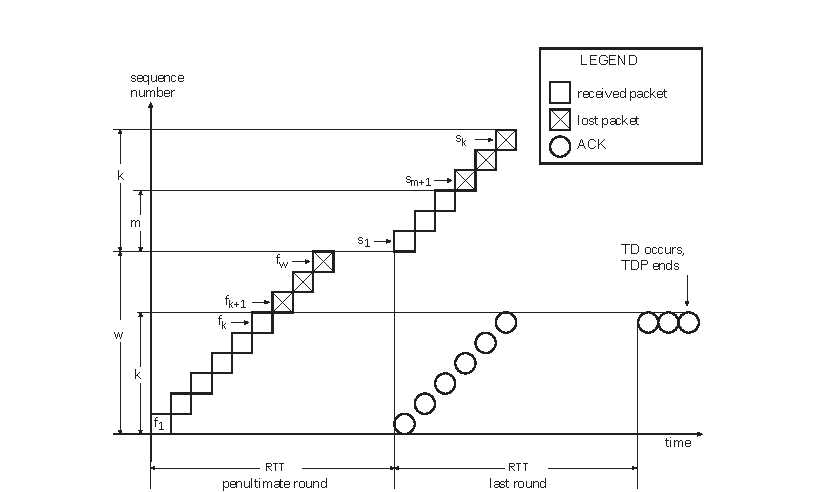
\includegraphics[scale=1.0]{figs/timeout2.pdf} 
\caption{Pacote e transmissões de ACKs precedendo uma indicação de perda}
\label{fig4}
\end{center}
\end{figure}

Nós começamos por derivar uma expressão para Q. Considere a rodada de pacotes onde uma indicação de perda ocorre; isso será referenciado como a penúltima rodada (ver figura \ref{fig4}, nessa figura cada ACK reconhece pacotes individuais). Deixe $w$ ser o tamanho da janela de congestionamento. Os pacotes $f_1..f_w$ são transmitidos na penúltima rodada. Os pacotes $f_1..f_k$ são reconhecidos e o pacote $f_{k+1}$ é o primeiro a ser perdido (ou não reconhecido). Assume-se que quando um pacote é perdido, todos os outros na sequência e na mesma rodada também são perdidos. Assim, todos os pacotes que seguem $f_{k+1}$ na penúltima rodada também são perdidos. Entretanto, como os pacotes $f_1..f_k$ são reconhecidos, então outros $k$ pacotes $s_1..s_k$ são transmitidos na próxima rodada, que é referenciada como a última rodada. Esta rodada de pacotes pode ter outra perda, diga-se $s_{m+1}$. Assim, $s_{m+2}..s_k$ também são perdidos na última rodada. Os $m$ pacotes transmitidos com sucesso na última rodada são respondidos por ACKs para o pacote $f_k$, que são contados como ACKs duplicados. Dessa maneira, o número de ACKs duplicados é igual ao número de pacotes recebidos com sucesso na última rodada. Se o número de ACKs é maior do que três, então ocorre uma indicação de perda por ACKs duplicados, senão, um timeout ocorre. Em ambos os casos, o período atual entre as perdas, TDP, finaliza. Denota-se por $A(w,k)$ a probabilidade que os primeiros $k$ pacotes sejam reconhecidos numa rodada de $w$ pacotes, dado que existe uma sequência de uma ou mais perdas na rodada. Então:

$$A(w, k) = \frac{(1-p)^kp}{1-(1-p)^w} $$

onde:

$p$ é a probabilidade de perda. \\
$(1-p)^k$ é a probabilidade de sucesso, k vezes. \\
$(1-p)^w$ é a probabilidade de sucesso, w vezes. \\
$1 - (1-p)^w$ é a probabilidade de uma ou mais perdas numa rodada de $w$ pacotes. \\

Também, define-se $C(n,m)$ como a probabilidade que $m$ pacotes sejam reconhecidos em sequência na última rodada (onde $n$ pacotes são transmitidos) e o resto dos pacotes na rodada, se houver, são perdidos. Então,

$$C(n,m) = \begin{cases} 
  (1-p)^mp,  \ \  m \leq n - 1 \ \ \ \ houve \ perda\\
  (1-p)^n,  \ \  m = n \ \ \ \ somente \ sucesso\\
\end{cases}
 $$

Então, $\hat{Q}(w)$, a probabilidade que uma perda numa janela de tamanho $w$ seja por timeout, é dada por:

$$\hat{Q}(w) = \begin{cases} 
  1,  \ \ se \ w \leq 3 \ \ \ \ n\tilde{a}o \ tem \ como \ ter \ TD, \ ent\tilde{a}o \ \acute{e} \ TO\\
  \underbrace{\sum_{k=0}^2A(w,k)}_{garante \ w \ > \ 3.} + \underbrace{\sum_{k=3}^wA(w,k)}_{houve \ perda.}.\underbrace{\sum_{m=0}^2C(k,m)}_{se \ m \ > \ 3 \ \acute{e} \ TD.},  \ \  caso \ contr\acute{a}rio \ \ \ \ \\
\end{cases}
 $$

Assim, um timeout ocorre se o número de pacotes transmitidos corretamente na penúltima rodada, $k$, é menor que três, ou se o número de pacotes transmitidos com sucesso na última rodada, $m$, é menor que três. Também, devido à suposição que o pacote $s_{m+1}$ é perdido independentemente do pacote $f_{k+1}$ (eles ocorrem em diferentes rodadas), a probabilidade que exista uma perda em $f_{k+1}$ na penúltima rodada e uma perda em $s_{m+1}$ na última rodada é igual a $A(w,k)*C(k,m)$.

Agora, iremos resolver o segundo caso de $\hat{Q}(w)$:

$$ X = \underbrace{\sum_{k=0}^2A(w,k)}_{(I)} + \underbrace{\sum_{k=3}^wA(w,k)}_{(II)}.\underbrace{\sum_{m=0}^2C(k,m)}_{(III)}$$

Tendo em mente que para uma PG finita de razão $\neq$ 1, o $\sum_{k=0}^nx^k = \dfrac{x^{n+1}-1}{x-1}$.

Para I, temos:

$$\sum_{k=0}^2A(w,k) =  \sum_{k=0}^2\frac{(1-p)^kp}{1-(1-p)^w}$$
$$ = \frac{p}{1-(1-p)^w} \cdot\sum_{k=0}^2(1-p)^k$$
$$ = \frac{p}{1-(1-p)^w}\cdot \frac{(1-p)^3 -1}{(1-p) - 1}\cdot\frac{(-1)}{(-1)}$$
$$ = \frac{p}{1-(1-p)^w} \cdot \frac{1 - (1-p)^3}{p}$$
$$ = \frac{1 - (1-p)^3}{1-(1-p)^w}$$

Para III, temos:

$$\sum_{m=0}^{2}C(k,m) = \sum_{m=0}^{2}(1-p)^mp $$
$$ = p \cdot \sum_{m=0}^{2}(1-p)^m $$
$$ = p \cdot \frac{(1-p)^3 - 1}{(1-p) - 1} $$
$$ = p \cdot \frac{1- (1-p)^3}{p} $$
$$ = 1- (1-p)^3 $$

Para II, temos: 

$$\sum_{k=3}^{w}A(w,k) =  \sum_{k=3}^{w}\frac{(1-p)^kp}{1-(1-p)^w}$$
$$ = \frac{p}{1-(1-p)^w} \cdot \underbrace{\sum_{k=3}^{w}(1-p)^k}_{(IV)} $$

Para IV, temos:

$$\sum_{k=3}^{w}(1-p)^k = \sum_{k=0}^{w}(1-p)^k - \sum_{k=0}^{2}(1-p)^k$$
$$= \frac{(1-p)^{w+1}-1}{(1-p)-1} - \frac{(1-p)^{3}-1}{(1-p)-1}$$
$$= \frac{1 - (1-p)^{w+1}}{p} - \frac{1 - (1-p)^{3}}{p}$$
$$= \frac{(1-p)^3 - (1-p)^{w+1}}{p}$$
$$= \frac{(1-p)^3 \cdot (1 - (1-p)^{w-2})}{p}$$

Voltando para II:

$$\frac{p}{1-(1-p)^w} \cdot \frac{(1-p)^3 \cdot (1 - (1-p)^{w-2})}{p} $$
$$ = \frac{(1-p)^3 \cdot (1 - (1-p)^{w-2})}{1-(1-p)^w} $$

Dessa maneira:

$$X = \frac{1- (1-p)^3}{1 - (1-p)^w} + \frac{(1-p)^3 \cdot (1 - (1-p)^{w-2})}{1-(1-p)^w} \cdot (1-(1-p)^3)$$
$$ = \frac{(1-(1-p)^3)\cdot (1 + (1-p)^3\cdot (1 - (1-p)^{w-2}))}{1 - (1-p)^w}$$

Portanto, 

$$ \hat{Q}(w) = min(1, \frac{(1-(1-p)^3)\cdot (1 + (1-p)^3\cdot (1 - (1-p)^{w-2}))}{1 - (1-p)^w}) $$

Agora, podemos aplicar a regra de L'Hopital para simplificarmos a segunda parte de $\hat{Q}(w)$, quando as perdas são tão pequenas que tendem a zero.

Para aplicarmos a regra de L'Hopital,  $f(x)$ e $g(x)$ precisam ser funções diferenciáveis, com $g'(x) \neq 0, \ \forall x$. Além disso, se $\lim_{x \to p}f(x) = 0$ e $\lim_{x \to p}g(x) = 0$, então, se existir $\lim_{x \to p}\frac{f'(x)}{g'(x)}$, temos que:

$$\lim_{x \to p}\frac{f(x)}{g(x)} = \lim_{x \to p}\frac{f'(x)}{g'(x)}$$

Quando as perdas de pacotes tendem a zero, podemos aplicar:

$$\lim_{p \to 0}\frac{(1-(1-p)^3)\cdot (1 + (1-p)^3\cdot (1 - (1-p)^{w-2}))}{1 - (1-p)^w} = x $$
$$x = \lim_{p \to 0}\frac{\overbrace{[(1-(1-p)^3)\cdot (1 + (1-p)^3\cdot (1 - (1-p)^{w-2}))]'}^{f'(x)}}{\underbrace{[1 - (1-p)^w]'}_{g'(x))}}$$

Para $f'(x)$, temos:

$$f'(x) = [(1-(1-p)^3)\cdot (1 + (1-p)^3\cdot (1 - (1-p)^{w-2}))]'$$
$$= (1-(1-p)^3)\cdot \underbrace{[(1 + (1-p)^3\cdot (1 - (1-p)^{w-2}))]'}_{(i)} + \underbrace{[(1-(1-p)^3)]'}_{(ii)} \cdot(1 + (1-p)^3\cdot (1 - (1-p)^{w-2}))$$

Para $i$, temos:

$$[(1 + (1-p)^3\cdot (1 - (1-p)^{w-2}))]' =  (1)' + [(1-p)^3\cdot (1 - (1-p)^{w-2})]'$$
$$=  0 + (1-p)^3\cdot \underbrace{[(1 - (1-p)^{w-2}))]'}_{(iii)} + [(1-p)^3]'\cdot (1 - (1-p)^{w-2})$$

Para $iii$, temos:

$$[(1 - (1-p)^{w-2}))]' = (1)' - [(1-p)^{w-2})]') $$
$$ = 0 - (w-2)(1-p)^{w-3})) $$
$$ = (2-w)(1-p)^{w-3} $$

Voltando para $i$:

$$ (1-p)^3\cdot (2-w)(1-p)^{w-3} + 3(1-p)^2\cdot (1 - (1-p)^{w-2})$$
$$= (1-p)^w(2-w) + 3(1-p)^2 - 3(1-p)^2(1-p)^{w-2}$$
$$= (1-p)^w(2-w) + 3(1-p)^2 - 3(1-p)^w$$
$$= (1-p)^w(2-w -3) + 3(1-p)^2$$
$$= (1-p)^w(-w -1) + 3(1-p)^2$$

Para $ii$, temos:

$$[1-(1-p)^3]' = 0 - [(1-p)^3]' $$
$$= - 3(1-p)^2 $$

Então, 

$$f'(x) = (1 - (1-p)^3)[(1-p)^w(-w-1) + 3(1-p)^2] - 3(1-p)^2(1+(1-p)^3(1-(1-p)^{w-2})) $$
$$= (1-p)^w(-w-1) + \cancel{3(1-p)^2} - (1-p)^{w+3}(-w-1) - 3(1-p)^5 \cancel{- 3(1-p)^2} - 3(1-p)^5(1-(1-p)^{w-2}) $$
$$= (1-p)^{w-1}[(1-p)(-w-1) - (1-p)^4(-w-1) - 3(1-p)^{6-w} - 3(1-p)^{6-w}(1-(1-p)^{w-2})]$$

Para $g'(x)$, temos:

$$g'(x) = [1 - (1-p)^w]' $$
$$ = (1)' - [(1-p)^w]' $$
$$ = 0 - w(1-p)^{w-1} $$
$$ = - w(1-p)^{w-1} $$

Portanto, 

$$\tiny{x = \lim_{p \to 0}\frac{\cancel{(1-p)^{w-1}}[(1-p)(-w-1) - (1-p)^4(-w-1) - 3(1-p)^{6-w} - 3(1-p)^{6-w}(1-(1-p)^{w-2})]}{- w\cancel{(1-p)^{w-1}}} }$$

Fazendo $p = 0$, temos:

$$x = \frac{[(1-0)(-w-1) - (1-0)^4(-w-1) - 3(1-0)^{6-w} - 3(1-0)^{6-w}(1-(1-0)^{w-2})]}{- w} $$
$$= \frac{\cancel{(1)(-w-1)} \cancel{- (1)(-w-1)} - 3(1) - \cancel{3(1)(0)}}{- w} $$
$$= \frac{- 3(1)}{- w} $$
$$= \frac{3}{w} $$

Numericamente nós achamos uma aproximação muito boa de $\hat{Q}$ que é:

$$\hat{Q}(w) \approx min(1, \frac{3}{w}) $$

Q, a probabilidade de que uma indicação de perda seja por timeout, é:

$$Q = \sum_{w=1}^{\infty}\hat{Q}(w)P[W = w] = E[\hat{Q}]$$

Nós aproximamos 

$$Q \approx \hat{Q}(E[W])$$

A próxima derivação a ser considerada é a de $E[Y^{TO}]$ ou $E[R]$. Para isso, precisamos da distribuição de probabilidade do número de timeouts em uma sequência de TO, dado que exista um TO. Observou-se que, em muitos dos \textit{traces} do TCP, um pacote é transmitido entre dois timeouts em sequência. Assim, uma sequência de $k$ TOs ocorre quando existem $k - 1$ perdas consecutivas (a primeira perda já foi contada) seguidas por um pacote transmitido corretamente. Consequentemente, o número de TOs numa sequência de TOs tem uma distribuição geométrica, e portanto

$$P[R = k] = \underbrace{p^{k-1}}_{k-1 \ perdas.} \cdot \underbrace{(1-p)}_{um \ sucesso.} $$

Tendo em vista que para uma PG infinita de razão $|x|<1, \ \sum_{k=1}^{\infty}kx^k = \frac{x}{(1-x)^2} $, nós podemos computar a média de R

$$E[R] = \sum_{k=1}^{\infty}kP[R=k]$$
$$= \sum_{k=1}^{\infty}kp^{k-1}(1-p)$$
$$= (1-p)\cdot \sum_{k=1}^{\infty}kp^{k-1}$$
$$= \frac{(1-p)}{p}\cdot \sum_{k=1}^{\infty}kp^{k}$$
$$= \frac{(1-p)}{p}\cdot \frac{p}{(1-p)^2}$$
$$= \frac{1}{(1-p)}$$

No próximo passo, nos concentramos no $E[Z^{TO}]$, a duração média de uma sequência de timeouts excluindo as retransmissões, que podem ser computadas de uma maneira parecida. Sabe-se que os primeiros seis timeouts em uma sequência tem o tamanho $2^{i-1}T_o$, $i = 1...6$, com todos os timeouts seguintes tendo tamanho $64T_o$. Então, a duração de uma sequência com $k$ timeouts é

$$L_k = \begin{cases} 
  (2^k - 1)T_o,  \ \  para \  k \leq 6 \\
  (63 + 64(k-6))T_o,  \ \ para  \ k \geq 7\\
\end{cases} $$

e a média de $Z^{TO}$ é

$$E[Z^{TO}] = \sum_{k=1}^{\infty}L_kP[R=k] $$
$$=  \sum_{k=1}^{6}(2^k -1)T_op^{k-1}(1-p) + \sum_{k=7}^{\infty}(63+64(k-6))T_op^{k-1}(1-p)$$
$$=  T_o(1-p) \cdot [\underbrace{\sum_{k=1}^{6}(2^k -1)p^{k-1}}_{(1)} + \underbrace{\sum_{k=7}^{\infty}(63+64(k-6))p^{k-1}}_{(2)}] $$

Para 2, temos:

$$\sum_{k=7}^{\infty}(63+64(k-6))p^{k-1} = \underbrace{\sum_{k=7}^{\infty}63p^{k-1}}_{(3)} + \underbrace{\sum_{k=7}^{\infty}64(k-6)p^{k-1}}_{(4)} $$

Para 3, temos:

$$\sum_{k=7}^{\infty}63p^{k-1} = \frac{63}{p}\cdot \sum_{k=7}^{\infty}p^{k} $$
$$ = \frac{63}{p}\cdot [\sum_{k=0}^{\infty}p^{k} - \sum_{k=0}^{6}p^{k}] $$
$$ = \frac{63}{p}\cdot [\frac{1}{(1-p)} - (1 + \frac{p - p^7}{1-p})] $$
$$ = \frac{63}{p}\cdot [\frac{1}{(1-p)} - (\frac{1 - p^7}{1-p})] $$
$$ = \frac{63}{p}\cdot [\frac{p^7}{(1-p)}] $$
$$ = \frac{63p^6}{(1-p)} $$

Para 4, temos:

$$\sum_{k=7}^{\infty}64(k-6)p^{k-1} =  \frac{64}{p} \cdot \sum_{k=7}^{\infty}(k-6)p^{k}$$
$$ =  \frac{64}{p} \cdot [\underbrace{\sum_{k=7}^{\infty}kp^{k}}_{(5)} - \underbrace{6 \cdot \sum_{k=7}^{\infty}p^{k}}_{(6)}]  $$

Para 5, temos:

$$\sum_{k=7}^{\infty}kp^{k} =  \sum_{k=1}^{\infty}kp^{k} - \sum_{k=1}^{6}kp^{k}$$
$$ =  \frac{p}{(1-p)^2} - \frac{p - 7p^7 + 6p^8}{(1-p)^2} $$
$$ =  \frac{7p^7 - 6p^8}{(1-p)^2} $$

Para 6 e aplicando o que vimos em 3, temos:

$$6 \cdot \sum_{k=7}^{\infty}p^{k} = \frac{6p^7}{(1-p)} $$

Voltando para 4, temos:

$$\frac{64}{p}\cdot [\frac{p}{(1-p)} \cdot (\frac{7p^6 - 6p^7}{(1-p)} - 6p^6] $$
$$= \frac{64}{(1-p)}\cdot [\frac{7p^6 - 6p^7}{(1-p)} - 6p^6] $$
$$= \frac{64p^6}{(1-p)}\cdot [\frac{7 - 6p}{(1-p)} - 6] $$
$$= \frac{64p^6}{(1-p)}\cdot \frac{7 - 6p - (6 - 6p)}{(1-p)} $$
$$= \frac{64p^6}{(1-p)^2} $$

Voltando para 2, temos:

$$ \frac{63p^6}{(1-p)} +  \frac{64p^6}{(1-p)^2}$$
$$= \frac{p^6}{(1-p)} \cdot (63 + \frac{64}{(1-p)}) $$
$$= \frac{p^6}{(1-p)} \cdot (\frac{63 - 63p + 64}{(1-p)}) $$
$$= \frac{p^6(127 - 63p)}{(1-p)^2} $$

Para 1, temos:

$$\sum_{k=1}^{6}(2^k -1)p^{k-1} = \frac{1}{p}\cdot \sum_{k=1}^{6}(2^k -1)p^{k}$$
$$ = \frac{1}{p}\cdot [\underbrace{\sum_{k=1}^{6}(2p)^{k}}_{(7)} - \underbrace{\sum_{k=1}^{6}p^{k}}_{(8)}]$$

Para 7, temos:

$$\sum_{k=1}^{6}(2p)^{k} = 2p + 4p^2 + 8p^3 + 16p^4 + 32p^5 + 64p^6 $$

Para 8, temos:

$$\sum_{k=1}^{6}p^{k} = \sum_{k=0}^{6}p^{k} - 1$$
$$= \frac{p^7 -1}{p-1}\cdot \frac{(-1)}{(-1)} - 1$$
$$= \frac{1 - p^7}{(1-p)} - 1$$
$$= \frac{1 - p^7 - (1-p)}{(1-p)} $$
$$= \frac{- p^7 +p}{(1-p)} $$

Voltando para 1, temos:

$$\frac{1}{p} \cdot [p(2 + 4p + 8p^2 + 16p^3 + 32p^4 64p^5) - p \cdot (\frac{-p^6 + 1}{1-p})] $$
$$= 2 + 4p + 8p^2 + 16p^3 + 32p^4 64p^5 + \frac{p^6 - 1}{1-p} $$
$$= \frac{2 - 2p + 4p - 4p^2 + 8p^2 - 8p^3 + 16p^3 - 16p^4 + 32p^4 - 32p^5 + 64p^5 - 64p^6 + p^6 -1}{1-p} $$
$$= \frac{1 + 2p + 4p^2 + 8p^3 + 16p^4 + 32p^5 - 63p^6}{1-p} $$

Portanto, temos que $E[Z^{TO}]$ é:

$$E[Z^{TO}] = T_o(1-p) \cdot [\frac{1}{(1-p)} \cdot (1 + 2p + 4p^2 + 8p^3 + 16p^4 + 32p^5 - 63p^6) + \frac{1}{(1-p)} \cdot (\frac{p^6(127 - 63p)}{(1-p)})] $$
$$ = T_o \cdot (1 + 2p + 4p^2 + 8p^3 + 16p^4 + 32p^5 - 63p^6 + \frac{p^6(127 - 63p)}{(1-p)}) $$
$$\textstyle{ = \frac{T_o(1 - p +2p - 2p^2 + 4p^2 - 4p^3 + 8p^3 - 8p^4 + 16p^4 - 16p^5 + 32p^5 -32p^6 - 63p^6 + 63p^7 + 127p^6 - 63p^7)}{1-p}}$$
$$ = T_o \cdot \frac{1+p+2p^2 + 4p^3 + 8p^4 + 16p^5 + 32p^6}{1-p}$$

Onde $f(p) = 1+p+2p^2 + 4p^3 + 8p^4 + 16p^5 + 32p^6$. Assim, 

$$E[Z^{TO}] =  T_o \cdot \frac{f(p)}{1-p}$$


Agora, munido de todas as derivações, podemos finalizar a taxa de transmissão TCP como:

$$ \overline{X}(p) = \frac{E[Y] + Q.E[R]}{E[A] + Q.E[Z^{TO}]}$$
$$ = \frac{\frac{1-p}{p}+E[W] + Q(E[W])\frac{1}{1-p} } { RTT(E[X] + 1) + Q(E[W])T_o\frac{f(p)}{1-p}} $$


%Este arquivo deve ser alterado pelos integrantes da respectiva equipe com o conteudo indicado abaixo.
\subsection{Limitação do tamanho da janela do destinatário}
%Equipe: Sergio Vieira, Wilson

% Livro: Seção 5.3.1, p.136

%Inserir no arquivo \textbf{janela\_destino.tex} a descrição da influência do tamanho da janela 
%do detinatário no modelo TCP.

A modificação final do modelo é incluir uma situação na qual o destinatário pode limitar o tamanho da janela do remetente. Isto ocorre quando o destinatário pode processar pacotes até uma taxa de recepção máxima, neste caso, o remetente não deve transmitir uma rajada de pacotes a uma taxa que prejudique a recepção do destinatário. Em consequência disto, durante o período sem indicação de perda, o tamanho da janela pode crescer até um tamanho máximo (Figura \ref{fig:max}). 

\begin{figure}[ht]
  \centering
  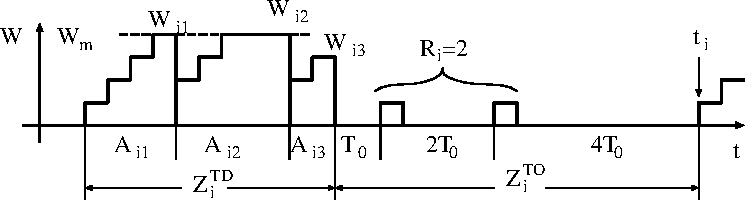
\includegraphics[scale=0.8]{figs/windowmax.pdf}
  \caption{Evolução do tamanho da janela limitada por um valor m
áximo}
  \label{fig:max}
\end{figure}

Denota-se $W_m$ como o limite imposto pelo destinatário para o tamanho máximo da janela e $W_u$ como o tamanho da janela sem restrições. Se $E[W_u]$ é menor que o limite da janela do destinatário, isto é, se $E[W_u]<W_m$, então a limitação da janela de recepção tem um efeito insignificante a longo prazo na vazão média do TCP, assim, como demonstrado anteriormente, $E[W_u]$
 é dado pela equação \ref{eq:wmax}. 

\begin{equation} \label{eq:wmax}
E[W_u]= 1 + \sqrt{\frac{8}{3p} - \frac{5}{3}}
\end{equation}

Se, entretanto, $W_m \leq E[W_u]$, a janela é considerada como sendo $E[W] \approx E[W_m]$. Desta maneira, como pode ser observado na Figura \ref{fig:limit}, em um período $Z_i^{TD}$ e em cada $TDP_i$, o tamanho da janela cresce linearmente até atingir um valor máximo $W_m$ em $U_i$ rodadas e permanece constante durante $V_i$ rodadas.

\begin{figure}[ht]
  \centering
  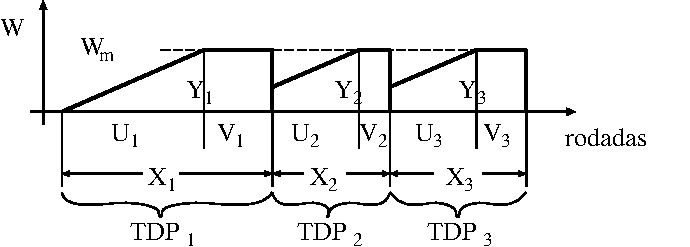
\includegraphics[scale=0.8]{figs/limit.pdf}
  \caption{Retransmissão rápida com limitação da janela}
  \label{fig:limit}
\end{figure}

Para determinar a quantidade de pacotes enviados no período $X_i$ basta calcular a área da figura formada durante $U_i$ rodadas (trapézio) mais a área da figura durante $V_i$ rodadas (retângulo). Assim a quantidade de pacotes $Y_i$ é dada por \ref{eq:pkts}.

\begin{equation} \label{eq:pkts}
Y_i=\frac{U_i(W_m + \frac{W_m}{2})}{2} + V_i \cdot W_m
\end{equation}

Desenvolvendo, tem-se:

\begin{align} \label{eq:EY1}
  \nonumber E[Y] &= \frac{W_mE[U]+\frac{W_mE[U]}{2}}{2} + W_mE[V]\\
  \nonumber     &= \frac{\frac{2W_mE[U]+W_mE[U]}{2}}{2} + W_mE[V]\\
       &= \frac{3W_mE[U]}{4} + W_mE[V]
\end{align}

Quando ocorre uma triplo ACK, a janela $W_m$ é dividida pela metade, assim, para que seu valor novamente atinja $W_m$ ela deve ser incrementada em $\frac{W_m}{2}$. No entanto, este acréscimo deve ocorrer dentro da rodada $U_i$, assim $W_m = \frac{W_m}{2} + U_i$, $\forall i \geq 2$ , desenvolvendo tem-se:

\begin{align} \label{eq:EY2}
  \nonumber W_m &= \frac{W_m}{2} + E[U]\\
  \nonumber     &= \frac{W_m+2E[U]}{2}\\
  \nonumber	2W_m - W_m &= 2E[U]\\
      E[U] &= \frac{W_m}{2}
\end{align} 

Substituindo $E[U]$ em \ref{eq:EY1}, tem-se:

\begin{align} \label{eq:EY3}
  \nonumber E[Y] &= \frac{3W_mE[U]}{4} + W_mE[V]\\
  \nonumber     &= \frac{3W_m\cdot \frac{W_m}{2}}{4} + W_mE[V]\\
      &= \frac{3W_m^2}{8} + W_mE[V]
\end{align}

Como o número de pacotes enviados em cada $TDP_i$ não se altera mesmo com um tamanho de janela limitado, o valor esperado de pacotes enviados é dado por $E[Y]=\frac{1-p}{p} + W_m$. Substituindo $E[Y]$ em \ref{eq:EY3} tem-se:

\begin{align} \label{eq:EY4}
  \nonumber \frac{1-p}{p} + W_m &= \frac{3}{8}W_m^2+W_mE[V]\\
  \nonumber \frac{ \frac{1-p}{p} + W_m }{W_m} &= \frac{ \frac{3}{8}W_m^2+W_mE[V] }{W_m}\\
  \nonumber \frac{1-p}{pW_m} + 1 &= \frac{3}{8}W_m+E[V]\\
  E[V] &= \frac{1-p}{pW_m} + 1 - \frac{3}{8}W_m
\end{align}

Finalmente, uma vez que $X_i=U_i+V_i$, temos:

\begin{align} \label{eq:EX}
  \nonumber E[X] &= E[U] + E[V]\\
  \nonumber &= \frac{W_m}{2} + \frac{1-p}{pW_m} + 1 - \frac{3}{8}W_m\\
  \nonumber &= \frac{W_m}{2} - \frac{3}{8}W_m + \frac{1-p}{pW_m} + 1\\
  \nonumber &= W_m(\frac{1}{2} - \frac{3}{8}) + \frac{1-p}{pW_m} + 1\\
  \nonumber &= \frac{1}{8}W_m + \frac{1-p}{pW_m} + 1\\
\end{align}

Para determinar a vazão do TCP levando-se em conta o tamanho máximo da janela substitui-se os valores de $E[X]$ na equação abaixo:

\begin{align} \label{eq:EX2}
  \nonumber  \overline{X}(p) &= \frac{\frac{1-p}{p}+E[W]+Q(E[W])\frac{1}{1-p}}{RTT(E[X]+1)+Q(E[W])T_0\frac{f(p)}{1-p}}\\
  \nonumber  \overline{X}(p) &= \frac{\frac{1-p}{p}+W_m+Q(W_m)\frac{1}{1-p}}{RTT(\frac{W_m}{8}+\frac{1-p}{pW_m}+1)+Q(E[W])T_0\frac{f(p)}{1-p}}
\end{align}

Portanto, o modelo completo da vazão do TCP é caracterizado por:

\begin{equation*}
\overline{X}(p)= 
\begin{cases} \dfrac{\frac{1-p}{p}+E[W]+Q(E[W])\frac{1}{1-p}}{RTT(\frac{E[W]}{2}+1)+Q(E[W])T_0\frac{f(p)}{1-p}}, & E[W_u]<W_m \\
\dfrac{\frac{1-p}{p}+W_m+Q(E[W_m])\frac{1}{1-p}}{RTT(\frac{W_m}{8}+\frac{1-p}{pW_m}+1)+Q(E[W_m])T_0\frac{f(p)}{1-p}}, & E[W_u]\approx W_m
\end{cases}
\label{eq:03}
\end{equation*}


\bibliographystyle{plain}	% (uses file "plain.bst")
\bibliography{tcp}		% expects file "myrefs.bib"


\end{document}
